\usepackage{amssymb}
\usetikzlibrary{calc}
\usetikzlibrary{shapes.geometric}
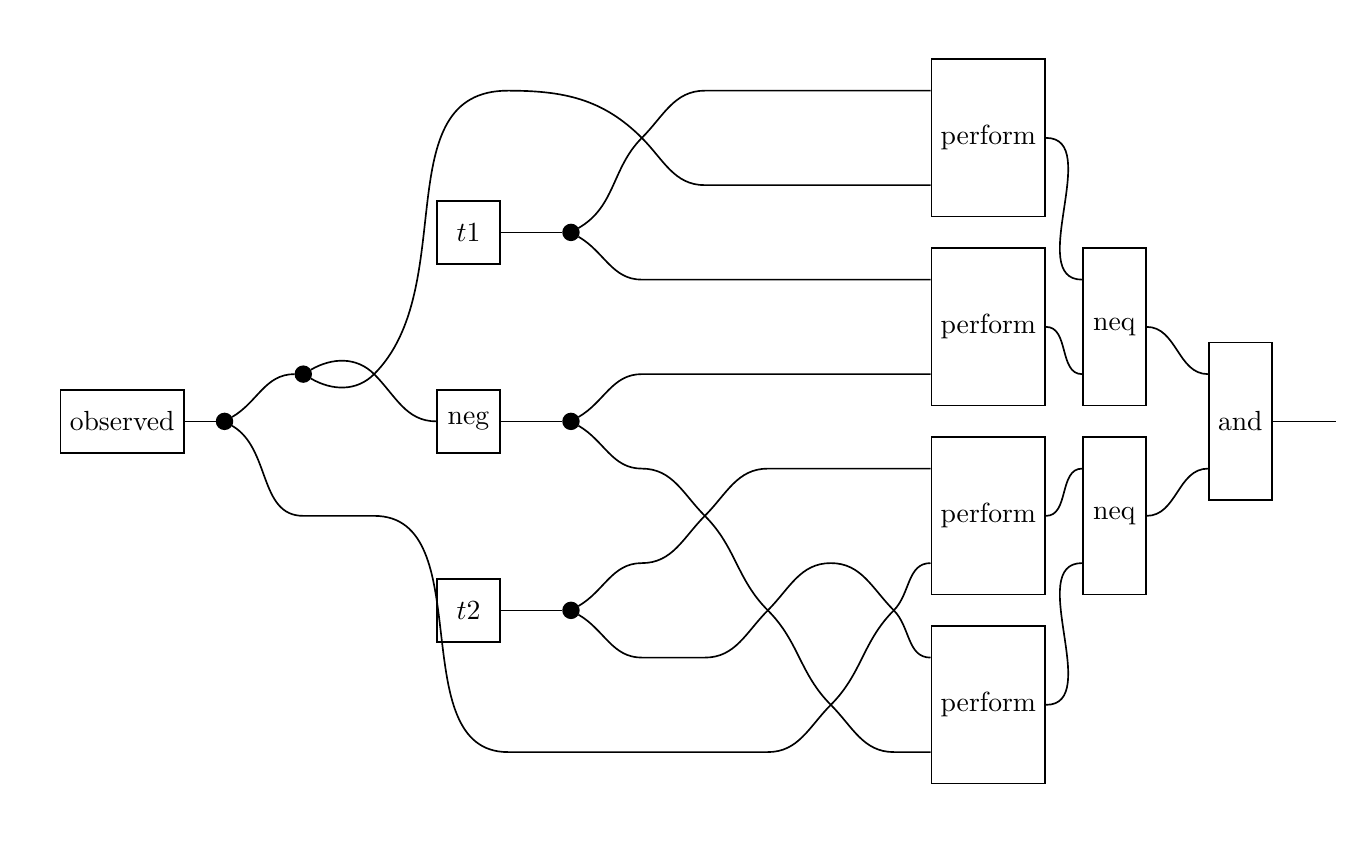
\begin{tikzpicture}[unit length/.code={{\newdimen\tikzunit}\setlength{\tikzunit}{#1}},unit length=4mm,x=\tikzunit,y=\tikzunit,semithick,box/.style={rectangle,draw,solid,sharp corners},junction/.style={circle,draw,fill,inner sep=0},outer box/.style={draw=none},wire/.style={draw}]
  \node[outer box,minimum width=41.5\tikzunit,minimum height=25\tikzunit] (root) at (0,0) {};
  \node[box,minimum size=2\tikzunit] (n3) at (-17.75,0) {$\mathrm{observed}$};
  \node[junction,minimum size=0.5\tikzunit] (n4) at (-14.5,0) {};
  \node[junction,minimum size=0.5\tikzunit] (n5) at (-12,1.5) {};
  \node[box,minimum size=2\tikzunit] (n6) at (-6.75,6) {$t1$};
  \node[junction,minimum size=0.5\tikzunit] (n7) at (-3.5,6) {};
  \node[box,minimum size=2\tikzunit] (n8) at (-6.75,0) {$\mathrm{neg}$};
  \node[junction,minimum size=0.5\tikzunit] (n9) at (-3.5,0) {};
  \node[box,minimum size=2\tikzunit] (n10) at (-6.75,-6) {$t2$};
  \node[junction,minimum size=0.5\tikzunit] (n11) at (-3.5,-6) {};
  \node[box,minimum width=2\tikzunit,minimum height=5\tikzunit] (n12) at (9.75,9) {$\mathrm{perform}$};
  \node[box,minimum width=2\tikzunit,minimum height=5\tikzunit] (n13) at (9.75,3) {$\mathrm{perform}$};
  \node[box,minimum width=2\tikzunit,minimum height=5\tikzunit] (n14) at (9.75,-3) {$\mathrm{perform}$};
  \node[box,minimum width=2\tikzunit,minimum height=5\tikzunit] (n15) at (9.75,-9) {$\mathrm{perform}$};
  \node[box,minimum width=2\tikzunit,minimum height=5\tikzunit] (n16) at (13.75,3) {$\mathrm{neq}$};
  \node[box,minimum width=2\tikzunit,minimum height=5\tikzunit] (n17) at (13.75,-3) {$\mathrm{neq}$};
  \node[box,minimum width=2\tikzunit,minimum height=5\tikzunit] (n18) at (17.75,0) {$\mathrm{and}$};
  \path[wire] (n3.east) to[out=0,in=180] (n4.180);
  \path[wire] (n4.30) to[out=30,in=180] (n5.180);
  \path[wire] (n4.-30) to[out=-30,in=180] (-12,-3) to[out=0,in=180] (-9.75,-3) to[out=0,in=180] (-5.5,-10.5) to[out=0,in=180] (-1.25,-10.5) to[out=0,in=180] (0.75,-10.5) to[out=0,in=180] (2.75,-10.5) to[out=0,in=-135] (4.75,-9) to[out=45,in=-135] (6.75,-6) to[out=45,in=-180] ($(n14.west)+(0,-1.5)$);
  \path[wire] (n5.30) to[out=30,in=135] (-9.75,1.5) to[out=-45,in=-180] (n8.west);
  \path[wire] (n5.-30) to[out=-30,in=-135] (-9.75,1.5) to[out=45,in=180] (-5.5,10.5) to[out=0,in=135] (-1.25,9) to[out=-45,in=180] (0.75,7.5) to[out=0,in=180] (2.75,7.5) to[out=0,in=180] (4.75,7.5) to[out=0,in=180] (6.75,7.5) to[out=0,in=-180] ($(n12.west)+(0,-1.5)$);
  \path[wire] (n6.east) to[out=0,in=180] (n7.180);
  \path[wire] (n7.30) to[out=30,in=-135] (-1.25,9) to[out=45,in=180] (0.75,10.5) to[out=0,in=180] (2.75,10.5) to[out=0,in=180] (4.75,10.5) to[out=0,in=180] (6.75,10.5) to[out=0,in=-180] ($(n12.west)+(0,1.5)$);
  \path[wire] (n7.-30) to[out=-30,in=180] (-1.25,4.5) to[out=0,in=180] (0.75,4.5) to[out=0,in=180] (2.75,4.5) to[out=0,in=180] (4.75,4.5) to[out=0,in=180] (6.75,4.5) to[out=0,in=-180] ($(n13.west)+(0,1.5)$);
  \path[wire] (n8.east) to[out=0,in=180] (n9.180);
  \path[wire] (n9.30) to[out=30,in=180] (-1.25,1.5) to[out=0,in=180] (0.75,1.5) to[out=0,in=180] (2.75,1.5) to[out=0,in=180] (4.75,1.5) to[out=0,in=180] (6.75,1.5) to[out=0,in=-180] ($(n13.west)+(0,-1.5)$);
  \path[wire] (n9.-30) to[out=-30,in=180] (-1.25,-1.5) to[out=0,in=135] (0.75,-3) to[out=-45,in=135] (2.75,-6) to[out=-45,in=135] (4.75,-9) to[out=-45,in=180] (6.75,-10.5) to[out=0,in=-180] ($(n15.west)+(0,-1.5)$);
  \path[wire] (n10.east) to[out=0,in=180] (n11.180);
  \path[wire] (n11.30) to[out=30,in=180] (-1.25,-4.5) to[out=0,in=-135] (0.75,-3) to[out=45,in=180] (2.75,-1.5) to[out=0,in=180] (4.75,-1.5) to[out=0,in=180] (6.75,-1.5) to[out=0,in=-180] ($(n14.west)+(0,1.5)$);
  \path[wire] (n11.-30) to[out=-30,in=180] (-1.25,-7.5) to[out=0,in=180] (0.75,-7.5) to[out=0,in=-135] (2.75,-6) to[out=45,in=180] (4.75,-4.5) to[out=0,in=135] (6.75,-6) to[out=-45,in=-180] ($(n15.west)+(0,1.5)$);
  \path[wire] (n12.east) to[out=0,in=-180] ($(n16.west)+(0,1.5)$);
  \path[wire] (n13.east) to[out=0,in=-180] ($(n16.west)+(0,-1.5)$);
  \path[wire] (n14.east) to[out=0,in=-180] ($(n17.west)+(0,1.5)$);
  \path[wire] (n15.east) to[out=0,in=-180] ($(n17.west)+(0,-1.5)$);
  \path[wire] (n16.east) to[out=0,in=-180] ($(n18.west)+(0,1.5)$);
  \path[wire] (n17.east) to[out=0,in=-180] ($(n18.west)+(0,-1.5)$);
  \path[wire] (n18.east) to[out=0,in=180] (root.east);
\end{tikzpicture}